\section{Adiabatic quantum computing \& quantum annealers}
%%%%%%%%%%%%%%%%%%%%%%%%%%%%%%%%%%%%
%%%%%%%%%%%%%%%%%%%%%%%%%%%%%%%%%%%%
%%%%%%%%%%%%%%%%%%%%%%%%%%%%%%%%%%%%
%%%%%%%%%%%%%%%%%%%%%%%%%%%%%%%%%%%%


 
In this section, we will present the example of vertex coloring problem using both D-Wave ocean stack as well as 1QBIT QUANTUM-READY™ SDK following the algorithm discussed in the section \ref{sec:annealing}.


%%%%%%%%%%%%%%%%%%%%%%%%%%%%%%%%%%%%%%%%%%
\subsection{Vertex Coloring with 1QBIT QUANTUM-READY™ SDK }
\begin{tcolorbox}[standard jigsaw,
    opacityback=0,  % this works only in combination with the key "standard jigsaw"
    boxrule=0.5pt,label={vertexcoloring}]
    {\bf Example: Vertex Coloring}
    \tcbline 
    Let’s solve the vertex coloring problem for the configuration shown in Figure \ref{fig:graph}
\end{tcolorbox}
\begin{figure}[h!]
\caption{Problem setting and sample solution of vertex coloring problem}
    \centering
    \begin{subfigure}[b]{0.4\textwidth}
        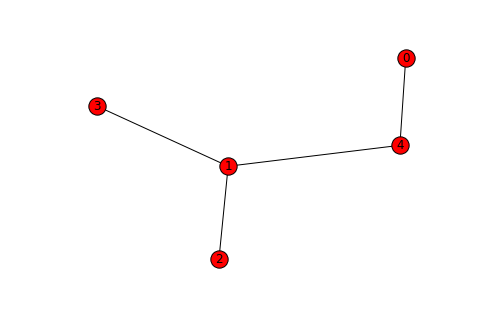
\includegraphics[width=\textwidth]{graph.png}
        \caption{Problem setting of the Vertex Coloring}
        \label{fig:graph}
    \end{subfigure}
     \begin{subfigure}[b]{0.4\textwidth}
        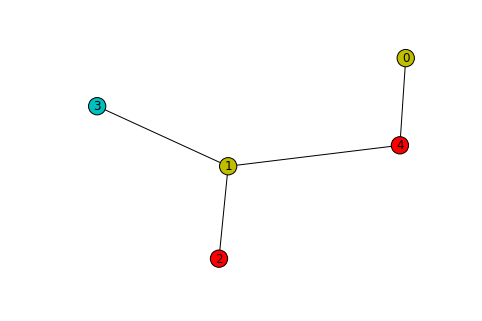
\includegraphics[width=\textwidth]{figures/colored.png}
        \caption{Final configuration after coloring}
        \label{fig:coloured}
    \end{subfigure}
\end{figure}
First we want to import the \texttt{networkx} and \texttt{matplotlib} library for the graph plotting.   
\begin{minted}{python}
import networkx as nx 
import matplotlib.pyplot as plt 

from qdk.binary_polynomial import * 
from qdk.common_solver_interface import * 
\end{minted}
The configuration of the coloring program is set by setting the nodes and neighbours.  The graph of the confifuration can be drawn.
\begin{minted}{python}
# Set the graph configuration by setting nodes and neighbours 
nodes = [0,1,2,3,4] 
neighbours = [(0,4),(1,2),(1,3),(1,4)] 
# Draw the graph configuration 
g = nx.Graph() 
g.add_nodes_from(nodes) 
g.add_edges_from(neighbours) 
pos = nx.spring_layout(g) 
nx.draw(g, pos=pos, with_labels=True, node_color='w', node_size=1000) 
plt.show() 
\end{minted}
As only one dimensional QUBO problem can be solved, the equation should be reduced to one dimension by reordering the index $n,k \rightarrow nK+k$.
\begin{minted}{python}
# Turn the two dimension index to one dimension
def d2tod1(n, k, K):  
    return n * K + k  
\end{minted}
Define the function to transfer the final solution to the colour label on the graph.
\begin{minted}{python}
# Function to color the final configuration
pallete = {0: 'r', 1: 'c', 2:'m', 3:'y'} 
def get_color(n, sol, K): 
    z = d2tod1(n, 0, K) 
    color = 0 
    for k in range(K): 
        if sol[z + k]: 
            break 
     return pallete[k] 
\end{minted}
Build the quadratic equation for vertex colouring problem:
\begin{equation}
H = \sum_{n=0}^{N-1}(1-\sum_{k=0}^{K-1}x_{nK+k})^2 + \sum_{(u,v)\in E}\sum_{k=0}^{K-1}x_{uK+k}x_{vK+k}
\end{equation}
\begin{minted}{python}
# Construct the quadratic equation 
builder = QuadraticBinaryPolynomialBuilder() 
qubo = builder.build_polynomial() 
N = 5 
K = 4
for n in range(N):
    builder.add_constant_term(1)
    for k in range(K):
        builder.add_term(-1, d2tod1(n,k,K))
    builder.power(2)
    t = builder.build_polynomial()
    qubo.sum(t)
    builder.reset()

for (u,v) in g.edges():
    for k in range(K): 
        builder.add_term(1, d2tod1(u,k,K), d2tod1(v,k,K))
        qubo.sum(builder.build_polynomial())
print (qubo) 
\end{minted}
We then set up the local solver and sample for 300 times
\begin{minted}{python}
solver = DWaveSolver() 
solver.solver.num_reads = 300 
sol = solver.minimize(qubo).peek_minimum_energy_solution().configuration 
\end{minted}
Finally we can draw the final configuration using the node\_color function defined.
\begin{minted}{python}
# Draw the final configuration with color applied
nx.draw(g, pos=pos, with_labels=True, nodelist=g.nodes(),  
node_color=[get_color(n, sol, K) for n in g.nodes()], node_size=1000) 
plt.show() 
\end{minted}

\begin{comment}
\inputminted{python}{code/dwave/colouring_qdk.txt}
\end{comment}

%%%%%%%%%%%%%%%%%%%%%%%%%%%%%%%%%%%%%%%%%
\subsection{Vertex Colouring with Ocean}
Following really similar steps, the same colouring problem can be implemented on D-Wave Ocean.

\inputminted{python}{code/dwave/colouring_ocean.txt}
%%%%%%%%%%%%%%%%%%

